\documentclass[10pt,a4paper]{article}
\usepackage[utf8]{inputenc}
\usepackage[italian]{babel}
\usepackage{amsmath}
\usepackage{amsfonts}
\usepackage{amssymb}
\usepackage{graphicx}
\usepackage[left=2cm,right=2cm,top=2cm,bottom=2cm]{geometry}

\author{Gruppo 1G.BT \\ Francesco Sacco, Lorenzo Cavuoti}
\title{Es03B: Amplificatore a transistor}

\begin{document}
	\maketitle
	\section{Verifica del punto di lavoro}
	Usando il multimetro digitale abbiamo misurato i valori delle resistenze e condensatori staccati dal circuito
\begin{itemize}
\item $R_1=(178.5\pm1.4)k\Omega$ 
\item $R_2=(17.65\pm0.14)k\Omega$ 
\item $R_C=(9.82\pm0.08)k\Omega$ 
\item $R_E=(1.014\pm0.008)k\Omega$
\item $C_{in}=(221\pm9)nF$
\item $C_{out}=(111\pm4)nF$
\end{itemize}
\\
\begin{enumerate}
\item Accendendo soltanto il generatore di ddp continua $V_{CC}=(19.97\pm0.10)$ abbiamo calcolato e misurato il punto di lavoro del transistor che risulta:
\begin{itemize}
\item $V_{CE,att}^Q = (7.3\pm0.4)V$ $I_{C,att}^Q = (1.17\pm0.03)mA$
\item $V_{CE,mis}^Q = (9.00\pm0.05)V$ $ I_{C,mis}^Q = (1.01\pm0.01)mA$
\end{itemize}
I due risultati non sono compatibili, tuttavia, come si vedrà anche in seguito, il circuito funziona correttamente, la discrepanza quindi si potrebbe attribuire a un errore nella presa dati o nei calcoli

\item Usando il multimetro digitale abbiamo misurato le tensioni ai terminali del transistor che risultano:
\begin{itemize}
\item $V_{B,mis} = 1.647\pm0.008$ $V_{E,mis} = 1.034\pm 0.005$ $V_{BE,mis} = 0.614\pm0.003$ $V_{C,mis} = 10.01\pm0.05$
\item $V_{B,att} \approx 1.7$ $V_{E,att} \approx 1.1$ $V_{BE,att} = 0.6$ $V_{C,att} \approx 10$\newline
Purtroppo è stato impossibile dare una stima accurata degli errori a causa dell'incognita su alcuni parametri del transistor
\end{itemize}
\item Sfruttando l'effetto transistor con $h_{fe}\approx 100$ abbiamo $I_B = I_C/h_{fe} \approx 10.1 \mu A$ dove $I_C$ è stata calcolata vedendo la ddp ai capi di $R_C$, inoltre sappiamo che $I_B = I_1-I_2 = (9\pm2)\mu A$ con $I_1$, $I_2$ calcolate prendendo la ddp su $R_1$, $R_2$ rispettivamente. L'errore risulta grande il quanto differenza di due misure simili, infatti $I_1=102.2\pm1.4\mu A$ $I_2=93.1\pm1.3\mu A$. Le due misure risultano compatibili, l'errore su 
\end{enumerate}
	
\section{Risposta a segnali sinusoidali a frequenza fissa}
In questo punto colleghiamo il generatore di funzioni al circuito con $f=6.24kHz$ e tutti i voltaggi sono misurati picco-picco
\begin{enumerate}
\item Vedendo $V_{in}$ e $V_{out}$ accoppiando l'oscilloscopio in AC notiamo che i due segnali sono in controfase con uno circa 10 volte l'altro (figura \ref{screen})
\begin{figure}
\centering
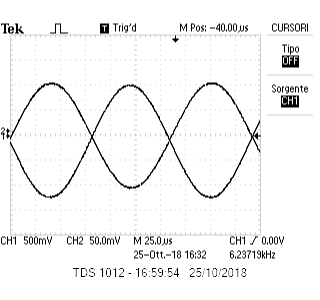
\includegraphics[scale=1]{3_1.png}
\caption{Inversione di fase tra ingresso e uscita, si notino le diverse scale su CH1 e CH2}
\label{screen} 
\end{figure}

\item Il guadagno atteso per piccoli segnali risulta $A_{V,att}=9.68\pm0.14$, per un onda sinusoidale con $V_{in} = (0.22\pm0.01)V$ si ha $V_{out} = (2.06\pm0.09)V$, $A_V=9.3\pm0.6$. Per verificare la linearità del sistema abbiamo preso un onda triangolare a diverse ampiezze. Con $V_{in} = (0.22\pm0.01)V$ si ha $V_{out} = (1.98\pm0.09V)$ $A_V=9.1\pm0.6$ e, con $V_{in} = 1.51\pm0.06V$  triangolare si ha $V_{out} = 13.7\pm0.6V$ $A_V=9.1\pm0.6$ i guadagni attesi risultano compatibili con quelli misurati.\newline
Inoltre la forma d'onda è rimasta pressocchè inalterata, quindi tutte le armoniche dello spettro della triangolare hanno trasformato allo stesso modo, questo dimostra la linearità del circuito tra $1$kHz e $10$kHz.\newline
\item Il circuito risulta lineare per $V_{in}$ minore di circa $1.5 V$ quindi $V_{out} \approx 18 V$ oltre questa ddp si ha il clipping, inizialmente questo spiana l'onda ma alzando ancora di più il voltaggio l'onda si inarca all'interno. 
\end{enumerate}		
		
\end{document}